\documentclass[11pt]{beamer}

\usetheme{epfl}
\usepackage{tikz}
\usetikzlibrary{positioning,arrows.meta}
\usetikzlibrary{calc,patterns,angles,quotes, fadings}
\usetikzlibrary{decorations}

\usepackage{media9}
\usepackage{amsmath}
\usepackage[thicklines]{cancel}
\usepackage{svg}
\newcommand{\citeapa}[1]{ {\tiny#1\par} }

% primary colors
\definecolor{tumblue}{RGB}{0,101,189} % Pantone 300
\definecolor{tumorange}{RGB}{227,114,34} % Pantone 158 - Orange


\begin{document}
	
	\title{Data-Driven Vegetation Modeling and Tackling Representation Shift}
	\subtitle{with Few-Shot Meta-Learning Methods}
	\author{Marc Russwurm}
	\labname{EPFL-ECEO}
	\date{\today}
	
	\logofilename{epfl/epfl_red.png}
	\titlepageimage{epfl/lacleman}
	\event{Deep Learning for Environment}
	\presentation{Representation Shift and Few-Shot Meta-Learning Methods}
	\speaker{Marc Russwurm}
	
	\begin{frame}[plain]
		\maketitle
	\end{frame}

	\begin{frame}{Structure}
		
		\begin{enumerate}
			\item Data-Driven Vegetation Modeling and 
			\begin{itemize}
				\item why is it meaningful
				\item data-driven verus model-driven approaches
			\end{itemize}
			\item<2-> Tackling Representation Shift 
			\begin{itemize}
				\item when does it arise?
				\item regional representations
			\end{itemize}
			\item<3> with Few-Shot Meta-Learning Methods
			\begin{itemize}
				\item seeing our remote sensing data as a dataset-of-datasets
				\item Model-agnostic meta-learning as one algorithm to tackle it.
			\end{itemize}
		\end{enumerate}
		
	\end{frame}

	\begin{frame}{Vegetation Modeling}
		\begin{tikzpicture}
			\node[fill=EPFLred, inner sep=1em, text=white, font=\bfseries]{Vegetation Modeling};
		\end{tikzpicture}
	\end{frame}


	\begin{frame}
		\frametitle{Why do we want to classify vegetation?}
		\begin{columns}
			\column{.5\textwidth}
			{\scriptsize
			\begin{description}
				\item[Zero Hunger] estimating the \textbf{crop yield} \& predict \textbf{food prices}, shortages.
				\item<2->[Climate Action] by monitoring \textbf{vegetation changes} over time (desertification).
				\item<3->[Life on Land] human life depends on \textbf{agriculture}, animal life on \textbf{biotopes}.
				%				\item Precision agriculture: sd
			\end{description}
			}
			\column{.5\textwidth}
			\includegraphics[width=\textwidth]{images/sdg_goals.pdf}
		\end{columns}
		
	\end{frame}

	\begin{frame}{Remote Sensing Data in Abundance}
		\begin{columns}[t]
			\column{.33\textwidth}
				MODIS
				\includemedia[
				width=\textwidth,
				activate=pageopen,
				addresource=mp4/apenne_modis_ndvi.mp4,
				flashvars={source=mp4/apenne_modis_ndvi.mp4&loop=true&
					autoPlay=true}
				]{\includegraphics[width=\textwidth]{mp4/apenne_modis_ndvi.png}}{mp4/apenne_modis_ndvi.mp4}
				{\tiny visualization \href{https://github.com/aaronpenne}{Aaron Penne Github}}
			
%				\vfill
%				\scriptsize daily, global scale, 36 bands (1km by 1km pixels)
			\column{.33\textwidth}
				Sentinel/Landsat
				\includemedia[
				width=\textwidth,
				activate=pageopen,
				addresource=mp4/sentinel2.mp4,
				flashvars={source=mp4/sentinel2.mp4&loop=true&
					autoPlay=true}
				]{\includegraphics[width=\textwidth]{mp4/sentinel2.png}}{mp4/sentinel2.mp4}
				{\tiny visualization ESA}
%				\vfill
%				\scriptsize 2-5 days, regional scale, 13 bands (10m by 10m pixels)
			\column{.33\textwidth}
				PlanetScope
				\includemedia[
				width=\textwidth,
				activate=pageopen,
				addresource=mp4/planet_denethor.mp4,
				flashvars={source=mp4/planet_denethor.mp4&loop=true&
					autoPlay=true}
				]{\includegraphics[width=\textwidth]{mp4/planet_denethor.png}}{mp4/planet_denethor.mp4}
				{\tiny DENETHOR dataset /\\ Kondmann et al., (2021)\par}
%				\vfill
%				\scriptsize daily, local scale, 4 bands (3m by 3m pixels)
		\end{columns}
	
		\vspace{1em}
		\small
	
		\begin{columns}
			\column{.33\textwidth}		
			\begin{itemize}
				\item daily/half-monthly
				\item 250m by 250m px
				\item 39 bands
			\end{itemize}	
			\column{.33\textwidth}
			\begin{itemize}
				\item 2-5 days
				\item 10m by 10m px
				\item 13 bands
			\end{itemize}
			\column{.33\textwidth}
			\begin{itemize}
				\item daily
				\item 3m by 3m pixels
				\item 4 bands
			\end{itemize}

	\end{columns}
	
		\vspace{3mm}
		\citeapa{Kondmann, et al., "DENETHOR: The DynamicEarthNET dataset for Harmonized, inter-Operable, analysis-Ready, daily crop monitoring from space.". NeurIPS Data Track (2021).}
	\end{frame}

	
	\begin{frame}
		\frametitle{Photosynthesis: Light $\rightarrow$ Life}
		%		\framesubtitle{Vegetation}
		
		\begin{columns}[b]
			
			\column{.5\textwidth}
			\includegraphics[width=\textwidth]{images/leaf_smallannot.pdf}
%			common remote sensing feature: $\text{NDVI} = \frac{\text{NIR} - \text{RED}}{\text{NIR} + \text{RED}}$ \\
			{\tiny Image adapted from wikipedia cc}
			%
			\column{.5\textwidth}
			\includegraphics[width=\textwidth]{images/reflectance_vegetation}
			\tiny Image from Roman et al., (2016)
		\end{columns}
		
		\normalsize
		
		\vspace{1em}
		Normalized Difference Vegetation Index.
		\vspace{1em}
		\begin{align}
			\text{NDVI}(\text{red}, \text{nir}) = \frac{\text{nir}-\text{red}}{\text{nir}+\text{red}}
		\end{align}
		
		\vfill
		
		\citeapa{Roman, A., \& Ursu, T. (2016). Multispectral satellite imagery and airborne laser scanning techniques for the detection of archaeological vegetation marks. Landsc. Archaeol. North. Front. Rom. Emp. Porolissum, 141-152.}
		
	\end{frame}

	\begin{frame}<presentation:1>
		\frametitle{Satellite Time Series}
		
		\begin{tikzpicture}[node distance=0em]
		\node(a) at (0,0){\includegraphics[width=10cm]{images/denethor/43647_Meadows_images}};
		\node(b)[below=0em of a]{\includegraphics[width=10cm]{images/denethor/82235_Wheat_images}};
		\visible<1>{
			\node(c)[below=1cm of b, xshift=-4em]{\includegraphics[width=.8\textwidth]{images/denethor/plots_2018.pdf}};
		}
	
		\visible<2>{
			\node(c)[below=1cm of b, xshift=-4em]{\includegraphics[width=.8\textwidth]{images/denethor/plotss2.pdf}};
		}
		\node(d)[right=-2em of c, yshift=1em]{\includegraphics[width=3cm]{images/denethor/map}};
		
		%\node[below=of c]{\includegraphics[width=.9\textwidth]{images/plotss2}};
		
		\definecolor{mpldefaultblue}{HTML}{1f77b4}
		%\coodinate (l1) at ($ (c) + (1,1) $);
%		\draw[Circle - , color=mpldefaultblue] ($ (c) + (-.45,1.6) $) -- ($ (b) + (-3.8,-.8) $); % requires \usetikzlibrary{arrows.meta} and calc
%		\draw[Circle - , color=mpldefaultblue] ($ (c) + (.78,1.6) $) -- ($ (b) + (-1.4,-.8) $);
%		\draw[Circle - , color=mpldefaultblue] ($ (c) + (1.38,1.6) $) -- ($ (b) + (1.6,-.8) $);
%		\draw[Circle - , color=mpldefaultblue] ($ (c) + (2.46,1.6) $) -- ($ (b) + (5,-.8) $);
		
		%\node[circle, draw] at (l1) {+};
		
		\end{tikzpicture}
		
		\citeapa{Kondmann, et al., "DENETHOR: The DynamicEarthNET dataset for Harmonized, inter-Operable, analysis-Ready, daily crop monitoring from space.". NeurIPS Data Track (2021).}
	\end{frame}

	\begin{frame}{Model-Driven Methods}
		\begin{columns}
			\column{.5\textwidth}
				\resizebox{\textwidth}{!}{
					\begin{tikzpicture}
					\node[label={above:\scriptsize growth stages of corn Mimic et al 2020}, inner sep=0](a){\includegraphics[width=6cm]{images/example/mimicetal2020_phenology_maize_}};
					
					\node[below=1em of a] (b){\includegraphics{images/example/NDVI}};
					
					\coordinate(left)  at ($(a.south west)+(-4.3em,0)$);
					\coordinate(right) at ($(a.south east)+(1.1em,0)$);
					
					\coordinate(veannot) at ($(left)!0.22!(right)$){};
					\coordinate(vtwoannot) at ($(left)!0.275!(right)$){};
					\coordinate(vfiveannot) at ($(left)!0.34!(right)$){};
					\coordinate(vtenannot) at ($(left)!0.42!(right)$){};
					\coordinate(btnnot) at ($(left)!0.5!(right)$){};
					\coordinate(rtwoannot) at ($(left)!0.6!(right)$){};
					\coordinate(rthreeannot) at ($(left)!0.7!(right)$){};
					\coordinate(rfiveannot) at ($(left)!0.8!(right)$){};
					\coordinate(harvestannot) at ($(left)!0.9!(right)$){};
					
					\coordinate(ve) at      ($ (b.center)+(-4em  ,1em) $);
					\coordinate(vtwo) at    ($ (b.center)+(-3em  ,1em) $);
					\coordinate(vfive) at   ($ (b.center)+(-2.5em,3em) $);
					\coordinate(vten) at    ($ (b.center)+(-2em  ,4em) $);
					\coordinate(bt) at      ($ (b.center)+(-1.5em,4.5em) $);
					\coordinate(rtwo) at    ($ (b.center)+(-1em  ,4.5em) $);
					\coordinate(rthree) at  ($ (b.center)+(-0em  ,2em) $);
					\coordinate(rfive) at   ($ (b.center)+(1.5em ,0.5em) $);
					\coordinate(harvest) at ($ (b.center)+(3em   ,0.5em) $);
					
					\draw[Circle-,tumorange](veannot)      -- (ve);
					\draw[Circle-,tumorange](vtwoannot)    -- (vtwo);
					\draw[Circle-,tumorange](vfiveannot)   -- (vfive);
					\draw[Circle-,tumorange](vtenannot)    -- (vten);
					\draw[Circle-,tumorange](btnnot)       -- (bt);
					\draw[Circle-,tumorange](rtwoannot)    -- (rtwo);
					\draw[Circle-,tumorange](rthreeannot)  -- (rthree);
					\draw[Circle-,tumorange](rfiveannot)   -- (rfive);
					\draw[Circle-,tumorange](harvestannot) -- (harvest);
					\end{tikzpicture}
				}
			\column{.5\textwidth}
				\includegraphics[width=\textwidth]{images/example/jointplot}
			
		\end{columns}
	
		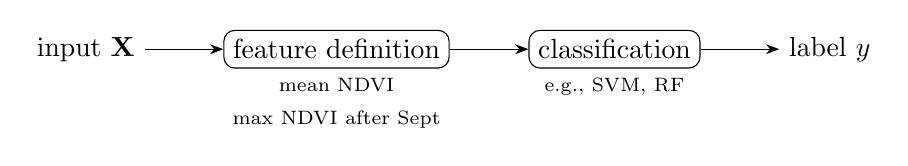
\begin{tikzpicture}
			\tikzstyle{process} = [draw, rounded corners]
			\node(x){input $\mathbf{X}$};
			\node[process, right=of x](f){feature definition};
			\node[process, right=of f](c){classification};
			\node[right=of c](y){label $y$};
			\draw[-Stealth](x) -- (f);
			\draw[-Stealth](f) -- (c);
			\draw[-Stealth](c) -- (y);
			\node[below=0cm of f, font=\scriptsize](a){mean NDVI};
			\node[below=0cm of a, font=\scriptsize](b){max NDVI after Sept};
			
			\node[below=0cm of c, font=\scriptsize](a){e.g., SVM, RF};
		\end{tikzpicture}
		
	\end{frame}

	
	\newcommand{\nn}{
		\tikzstyle{proba} = [circle, draw=white, inner sep=2.5pt, fill=rouge]
		\begin{tikzpicture}[scale=0.5, rotate=0, baseline=-.25em, minimum width=0cm, minimum height=0cm]
		\node[proba](a0) at (0,-1){};
		\node[proba](a1) at (0,0){};
		\node[proba](a2) at (0,1){};
		
		\node[proba](b0) at (1,-0.5){};
		\node[proba](b1) at (1,0.5){};
		
		\draw[-] (a0) -- (b0);
		\draw[-] (a1) -- (b0);
		\draw[-] (a2) -- (b0);
		
		\draw[-] (a0) -- (b1);
		\draw[-] (a1) -- (b1);
		\draw[-] (a2) -- (b1);
		
		%	\node[fit=(a0)(a2)(b1)](node name){};
		
		\end{tikzpicture}
	}

	\begin{frame}{Data-Driven Methods}
		
		
		\centering
		
		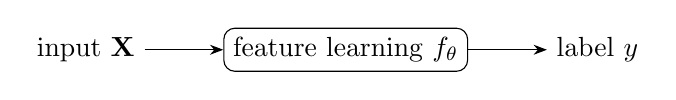
\begin{tikzpicture}
			\tikzstyle{process} = [draw, rounded corners]
			\node(x){input $\mathbf{X}$};
			\node[process, right=of x](f){feature learning $f_\mathbf{\theta}$ \nn};
			\node[right=of f](y){label $y$};
			\draw[-Stealth](x) -- (f);
			\draw[-Stealth](f) -- (y);
		\end{tikzpicture}
		
		\vfill
		
		
		\resizebox{\textwidth}{!}{
			\input{tikzfigures/NN-transformations.tikz}
		}
		
	\end{frame}
		
	\begin{frame}{Domain and Task}
		
		\centering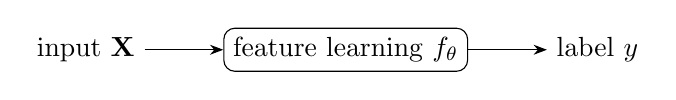
\begin{tikzpicture}
			\tikzstyle{process} = [draw, rounded corners]
			\node(x){input $\mathbf{X}$};
			\node[process, right=of x](f){feature learning $f_\mathbf{\theta}$ \nn};
			\node[right=of f](y){label $y$};
			\draw[-Stealth](x) -- (f);
			\draw[-Stealth](f) -- (y);
		\end{tikzpicture}
		
		\vspace{2cm}
		
		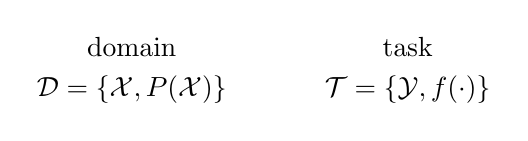
\begin{tikzpicture}
			\node[label=domain](domain){$\mathcal{D} = \{\mathcal{X}, P(\mathcal{X})\}$};
			\node[label=task, right=of domain](task){$\mathcal{T} = \{\mathcal{Y}, f(\cdot)\}$};
		\end{tikzpicture}
		\vfill\tiny
		\citeapa{Pan, S. J., \& Yang, Q. (2009). A survey on transfer learning. IEEE Transactions on knowledge and data engineering, 22(10), 1345-1359.}
	\end{frame}

	\begin{frame}
		\frametitle{I.I.D assumption}
		

		
		we use \textbf{independent}
		\begin{align*}
			\theta^\ast &= \arg\max_\theta \prod_{i} q(y_i \vert X_i)  \\
			&= \arg\max_\theta \sum_{i} -y_i \log f_\theta(X_i)
		\end{align*}
		 and \textbf{identically} distributed (i.i.d) samples
		 \begin{align}
		 	X_i,y_i \sim p(X, Y)	
		 \end{align}
		 from a datasets
		 \begin{align}
		 	\{X_i,y_i\}_i^N
		 \end{align}
		
	\end{frame}


	\begin{frame}{Representation Shift}
		\includegraphics[width=\textwidth]{images/countries_globe}
	\end{frame}
	
	\begin{frame}{Domain and Task}
		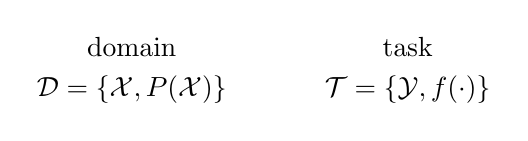
\begin{tikzpicture}
		\node[label=domain](domain){$\mathcal{D} = \{\mathcal{X}, P(\mathcal{X})\}$};
		\node[label=task, right=of domain](task){$\mathcal{T} = \{\mathcal{Y}, f(\cdot)\}$};
		\end{tikzpicture}
		\vfill\tiny
		\citeapa{Pan, S. J., \& Yang, Q. (2009). A survey on transfer learning. IEEE Transactions on knowledge and data engineering, 22(10), 1345-1359.}
		
	\end{frame}

	\begin{frame}{Shift in Remote Sensing Data}
		\includegraphics[width=.9\textwidth]{images/Sen12ms_distribution_shift}
		
		\citeapa{Rußwurm, M., Wang, S., Korner, M., \& Lobell, D. (2020). Meta-learning for few-shot land cover classification. In Proceedings of the ieee/cvf conference on computer vision and pattern recognition workshops (pp. 200-201).}
	\end{frame}
	
	
	\begin{frame}{A Frame Title}
		
		\begin{columns}
			\column{.5\textwidth}
			
			
			This is the frame content
			\begin{itemize}
				\item with some itemize objects
				\item and another one
			\end{itemize}
			
			Enumerates should work too
			\begin{enumerate}
				\item one
				\item two
			\end{enumerate}
		
			\column{.5\textwidth}
			
			A second column with other content, maybe more text, or something \emph{emphasized}. For more, highlight in \emphred{red} or \emphblue{blue}.
			
			
			
		\end{columns}
		
	\end{frame}

		
		\begin{frame}<presentation:9,13,14,15>%1-9,
			\frametitle{Deep Neural Networks}
			\centering
			
			\newcommand{\V}[1]{\ensuremath{\mathsymbol{\lowercase{#1}}}}
\newcommand{\M}[1]{\ensuremath{\mathsymbol{\uppercase{#1}}}}
%
%\newcommand{\mathbf{w}}{\ensuremath{\M{W}}}
%\newcommand{\mathbf{w}}{\ensuremath{\M{W}}}
\newcommand{\VBias}{\ensuremath{\V{b}}}
\newcommand{\VInput}{\DataVec}
\newcommand{\VHidden}{\ensuremath{\V{h}}}
\newcommand{\FActivation}{\ensuremath{\sigma}}
\newcommand{\VCellState}{\ensuremath{\V{c}}}
\newcommand{\VForgetGate}{\ensuremath{\V{f}}}
\newcommand{\VModulationGate}{\ensuremath{\V{j}}}
\newcommand{\VInputGate}{\ensuremath{\V{i}}}
\newcommand{\VOutputGate}{\ensuremath{\V{o}}}


\tikzstyle{circ} = [circle, draw=white, fill=tumblue, inner sep=1pt]
\newcommand{\fcn}{
	\begin{tikzpicture}[scale=0.2, rotate=0, baseline=-.25em, inner sep=1pt]
	\node[circ](a0) at (0,-1){};
	\node[circ](a1) at (0,0){};
	\node[circ](a2) at (0,1){};
	
	\node[circ](b0) at (1,-0.5){};
	\node[circ](b1) at (1,0.5){};
	
	\draw[-] (a0) -- (b0);
	\draw[-] (a1) -- (b0);
	\draw[-] (a2) -- (b0);
	
	\draw[-] (a0) -- (b1);
	\draw[-] (a1) -- (b1);
	\draw[-] (a2) -- (b1);
	
	\end{tikzpicture}
}


\newcommand{\earth}{
	\begin{tikzpicture}[baseline=-.25em, inner sep=0]
	\node{\includegraphics[width=8mm]{images/icons/earth}};
	\end{tikzpicture}
}

\newcommand{\sat}{
	\begin{tikzpicture}[baseline=-.25em, inner sep=0]
	\node[rotate=270,anchor=center]{\includegraphics[width=8mm]{images/icons/sat2}};
	\end{tikzpicture}
}

\newcommand{\hidden}[1]{
	\begin{tikzpicture}[scale=.1, baseline=-.25em]	
	%\draw[step=1.0,black,thin] (0,0) grid (#1,1);
	\foreach \i in {1,...,#1}{
		\node[circle, draw=white, fill=tumbluelight, inner sep=1pt] at (\i,0){};
	}
	\end{tikzpicture}
}

\newcommand{\drawvector}[1]{
	\begin{tikzpicture}[scale=.1, baseline=-.25em]	
	%\draw[step=1.0,black,thin] (0,0) grid (#1,1);
	\foreach \i in {1,...,#1}{
		\node[circ] at (\i,0){};
	}
	\end{tikzpicture}
}
\tikzstyle{proba} = [circle, draw=tumgray, inner sep=2.5pt, fill=tumorange]
\newcommand{\drawprobas}[5]{
	\begin{tikzpicture}[scale=.3, baseline=-.25em]	
	
	\node[proba, fill=tumblue!#1] at (0,-2){};
	\node[proba, fill=tumblue!#2] at (0,-1){};
	\node[proba, fill=tumblue!#3] at (0,-0){};
	\node[proba, fill=tumblue!#4] at (0,1){};
	\node[proba, fill=tumblue!#5] at (0,2){};
	\end{tikzpicture}
}



\newcommand{\vegetationsmodell}{
	\begin{tikzpicture}[scale=0.5, rotate=0, baseline=-.25em, minimum width=0cm, minimum height=0cm]
	\node[proba](a0) at (0,-1){};
	\node[proba](a1) at (0,0){};
	\node[proba](a2) at (0,1){};
	
	\node[proba](b0) at (1,-0.5){};
	\node[proba](b1) at (1,0.5){};
	
	\draw[-] (a0) -- (b0);
	\draw[-] (a1) -- (b0);
	\draw[-] (a2) -- (b0);
	
	\draw[-] (a0) -- (b1);
	\draw[-] (a1) -- (b1);
	\draw[-] (a2) -- (b1);
	
	%	\node[fit=(a0)(a2)(b1)](node name){};
	
	\end{tikzpicture}
}

\tikzstyle{tsmark} = [mark=|,mark size=2pt]

\colorlet{tumgray}{gray}
\colorlet{tumorange}{carotte}
\colorlet{tumblue}{leman}
\colorlet{tumbluedark}{canard}


\begin{tikzpicture}[node distance=.1em]
			\node[minimum width=1cm, minimum height=1.5cm, draw,rounded corners](veg) at (0,0){\vegetationsmodell};
			\coordinate[below=1em of veg](labelreference);
			\node(annotveg) at (labelreference){$f_{{\mathbf{w}}}$};
			\visible<1>{
				\node[above=2em of veg, font=\small, xshift=4em, text width=17em](annotf){\textbf{{\Large \color{tumblue}differentiable} non-linear function} \\ width randomly initialized weights $\mathbf{w}$};
				\draw[-stealth] (annotf) -- (veg);
			}
			\node[right=1em of veg, inner sep=0](input){%
				%		$\left(
				\only<1-12>{%
					$\mathbf{X}$%\rawtimeseriestwo{12-71456800.csv}%
				}%
				\only<0>{%9-12
					\begin{tikzpicture}[baseline=-1.5em, xscale=0.3, yscale=-.3]
					\foreach \x in {0,...,15}{
						\node[draw=tumgraylight, circle, fill=b2color, text=white, text opacity=1, font=\small, inner sep=2.5pt](d) at (\x,0){};
						\node[draw=tumgraylight, circle, fill=b3color, text=white, text opacity=1, font=\small, inner sep=2.5pt](d) at (\x,1){};
						\node[draw=tumgraylight, circle, fill=b4color, text=white, text opacity=1, font=\small, inner sep=2.5pt](d) at (\x,2){};
						\node[draw=tumgraylight, circle, fill=b5color, text=white, text opacity=1, font=\small, inner sep=2.5pt](d) at (\x,3){};
						\node[draw=tumgraylight, circle, fill=b6color, text=white, text opacity=1, font=\small, inner sep=2.5pt](d) at (\x,4){};
					}
					\end{tikzpicture}%
				}%
				\only<13-14>{
					\begin{tikzpicture}
					\node[draw, rounded corners, minimum width=1cm, minimum height=1.5cm](preproc){\includegraphics[width=.8cm]{images/icons/gears}};
					\node[right=1.5em of preproc](input){$\mathbf{X}$};%\rawtimeseriestwo{12-71456800_raw.csv}
					\node[font=\huge,left=0em of input, inner sep=0](bopen){$\Bigg($};
					\node[font=\huge, right=0em of input, inner sep=0](bopen){$\Bigg)$};
					\end{tikzpicture}
				}
				\only<15>{
					$\mathbf{X}$%\rawtimeseriestwo{12-71456800_raw.csv}
				}
			};% \rawtimeseries{prep77770412.csv}
			\only<13,14>{
				\node[right=1.5em of annotveg]{$f_{{\mathbf{w}}_\text{preproc}}$};
			}
			
			
			\node(annotinput) at (labelreference -| input){$\mathbf{X}$};
			\node[font=\huge,left=0em of input, inner sep=0](bopen){$\Bigg($};
			\node[font=\huge, right=0em of input, inner sep=0](bopen){$\Bigg)$};
			\node[left= of veg, font=\huge](equals){$=$};
			\only<-5>{\node[left= of equals](probas){\drawprobas{10}{30}{10}{20}{10}};}
			\visible<5>{\node[left= of equals](probas){\drawprobas{20}{30}{50}{20}{30}};}
			\visible<6>{\node[left= of equals](probas){\drawprobas{30}{40}{30}{50}{20}};}
			\visible<7>{\node[left= of equals](probas){\drawprobas{20}{20}{20}{80}{10}};}
			\visible<8->{\node[left= of equals](probas){\drawprobas{10}{30}{10}{100}{10}};}
			\node(annotprobas) at (labelreference -| probas){$\hat{y}$};
			\visible<2->{
				\node[left= 5em of probas](gt){\drawprobas{0}{0}{0}{100}{0}};
				\node(annotgt) at (labelreference -| gt){$\mathbf{y}$};
			}
			\visible<3->{
				\draw[stealth-stealth] (gt) -- node[midway,above](loss){$\mathcal{L}(\mathbf{y},\hat{y})$} (probas);
			}
			
			
			\visible<4->{\draw[-stealth] (loss)  to [out=60,in=135,looseness=1] node[midway,above]{${\mathbf{w}} \leftarrow \mathbf{w} - \frac{\partial \mathcal{L}}{\partial {\mathbf{w}}}$} (veg);}
			
			
			\only<9-12>{
				\node[above=10em of annotinput, font=\Large\bfseries, text=white, fill=tumbluedark, rounded corners](e1){End};
				\node[above=10em of annotgt, font=\Large\bfseries, text=white, fill=tumbluedark, rounded corners](e2){End};
				\node[above=10em of annotveg, text=white, fill=tumbluedark, font=\Large\bfseries, rounded corners](to){to};
				\draw[thick, tumbluedark] (e1) -- (to) -- (e2);
			}
			
			\only<10>{
				\node[below=of annotinput]{Satellite Time Series};
				\node[below=of annotgt]{Crop Types};
			}
			
			\only<11>{
				\node[below=of annotinput]{Images (single Band)};
				\node[below=of annotgt]{Cats and Dogs};
			}
			\only<12>{
				\node[below=of annotinput]{Text and Language};
				\node[below=of annotgt]{Sentiment};
			}
			
			\only<14>{
				\coordinate(fpreproc) at ($ (veg)+(3.5em,0) $);
				
				\draw[-stealth, dotted, red, thick] (loss)  to [out=-60,in=-135,looseness=1] node[midway,below]{\xcancel{$\frac{\partial \mathcal{L}}{\partial {\mathbf{w}}_\text{preproc}}$}} ($ (fpreproc)+(0,-2.3em) $);
				
				\node[above right=6em of fpreproc](a){$\mathbf{w}_\text{sel}$: start/end of vegetation period};
				\node[below right=6em of fpreproc](b){$\mathbf{w}_\text{atm}$: atmospheric parameters};
				\node[below right=7em and 2em of fpreproc, text width=14em](c){$\mathbf{w}_\text{cl}$: cloud classifier trained on different training set};
				\draw[-stealth, shorten >=4em] (a.south west) -- (fpreproc);
				\draw[-stealth, shorten >=4em] (b.north west) -- (fpreproc);
				\draw[-stealth, shorten >=4em] (c.north west) -- (fpreproc);
			}
			
		\end{tikzpicture}
	\end{frame}

	\begin{frame}{Colors}
		\centering
		\begin{tikzpicture}[xscale=2.6, yscale=-2]
		\tikzstyle{colorbox} = [minimum width=1.8cm, minimum height=1.8cm, text width=1.5cm, font=\scriptsize]
		
		\node(rouge) at (0,0)[fill=rouge,text=white, colorbox]{rouge};
		\node(leman) at (0,1)[fill=leman,text=white, colorbox]{leman};
		\node(grosseille) at (0,2)[fill=grosseille,text=white, colorbox]{grosseille};
		\node(canard) at (0,3)[fill=canard,text=white, colorbox]{canard};
		\node(montrose) at (1,0)[fill=montrose,text=white, colorbox]{montrose};
		\node(perle) at (1,1)[fill=perle,text=white, colorbox]{perle};
		\node(vertedeau) at (1,2)[fill=vertedeau,text=white, colorbox]{vertedeau};
		\node(rose) at (1,3)[fill=rose,text=white, colorbox]{rose};
		\node(acier) at (2,0)[fill=acier,text=white, colorbox]{acier};
		\node(soufre) at (2,1)[fill=soufre,text=white, colorbox]{soufre};
		\node(carotte) at (2,2)[fill=carotte,text=white, colorbox]{carotte};
		\node(zinzolin) at (2,3)[fill=zinzolin,text=white, colorbox]{zinzolin};
		\node(chartreuse) at (3,0)[fill=chartreuse,text=white, colorbox]{chartreuse};
		\node(marron) at (3,1)[fill=marron,text=white, colorbox]{marron};
		\node(ardoise) at (3,2)[fill=ardoise,text=white, colorbox]{ardoise};
		\node(taupe) at (3,3)[fill=taupe,text=white, colorbox]{taupe};
		
		\end{tikzpicture}
		
		
\end{frame}

\end{document}